\documentclass[a4paper,11pt]{report}
\usepackage{isolatin1}
\usepackage{amssymb}
\usepackage{epsfig}

\author{Tommy Petersen}

\title{Notes on an agent control algorithm based on a suffix tree}

\begin{document}

\maketitle

\newcommand{\R}{\mathbb{R}}
\newcommand{\Q}{\mathbb{Q}}
\newcommand{\Z}{\mathbb{Z}}
\newcommand{\N}{\mathbb{N}}

\newtheorem{lemma}{Lemma}[section]
\newtheorem{proposition}{Proposition}[section]
\newtheorem{theorem}{Theorem}[section]
\newtheorem{corollary}{Corollary}[section]
\newtheorem{algorithm}{Algorithm}[section]
\newtheorem{definition}{Definition}[section]
\newtheorem{example}{Example}[section]

\tableofcontents

\chapter{Suffix tree}
\section{Incremental update of the suffix tree}
Let $s$ be a string of symbols over a $k$-alphabet, and let $s^\prime := s + \alpha$ be $s$ concatenated with the
symbol $\alpha$. Let $T$ be the suffix tree for $s$ and let $T^\prime$ be the suffix tree for $s^\prime$. The question
is how to modify $T$ to get $T^\prime$ when incrementing $s$ with $\alpha$. This is the incremental update of the
suffix tree.

Let $\kappa$ be the prefix code for $s$ and let $\kappa^\prime$ be the prefix code for $s^\prime$. Since the context
set for $s$ cannot ``move to the left'' when adding the symbol $\alpha$, it follows that
for every suffix $s_i$ in $s$ that is encoded in $\kappa$ the corresponding suffix $s_i^\prime := s_i + \alpha$ in
$s^\prime$ is encoded in $\kappa^\prime$. Furthermore, since $\kappa$ is a shortest prefix code it follows that every
codeword, $\kappa_i$, in $\kappa$ is a prefix of the corresponding codeword, $\kappa_i^\prime$, in $\kappa^\prime$.
So, in $\kappa^\prime$, some of the codewords in $\kappa$ have been expanded (to the right), some have remained as they
were, but none have disappeared and none have shrunk.

The number of codewords, $|\kappa^\prime|$, in $\kappa^\prime$ are greater than or equal to the number of codewords,
$|\kappa|$, in $\kappa$. Let $N := |\kappa^\prime| - |\kappa|$ be the difference between $|\kappa^\prime|$ and $|\kappa|$,
then $N$ is either zero or strictly greater than zero.

If $N$ is zero, then $\kappa^\prime$ is identical to $\kappa$, because the same suffixes are encoded, and they are already
encoded in the shortest prefix code, $\kappa$.

If $N$ is strictly greater than zero, then a consecutive sequence of suffixes have been encoded by $\kappa^\prime$
additionally to the suffixes encoded by $\kappa$. The largest of the new suffixes encoded by $\kappa^\prime$ has an index
that is one greater than the index of the smallest suffix encoded by $\kappa$. The smallest of the new suffixes encoded by
$\kappa^\prime$ has an index that is one smaller than the index of the largest suffix in the context set of $s^\prime$.
Since each of these new suffixes were not encoded before adding $\alpha$ to $s$ it follows that each of the new codes
must be of the form $\gamma_i \alpha$, where $\gamma_i$ is in the context set of $s$. Denoting the set of new codewords
$\gamma$, we can write it as
$$
\gamma = \{\gamma_1 \alpha, \gamma_2 \alpha, \ldots, \gamma_N \alpha\}
$$
where the indexes are local to the new encodings, not global indexes in $s^\prime$.

The new code, $\kappa^\prime$, can be summarized by the following list;\hfill\break
\vskip0.5cm\noindent
$\kappa_1^\prime$\hfill\break
$\kappa_2^\prime$\hfill\break
$.$\hfill\break
$.$\hfill\break
$.$\hfill\break
$\kappa_I^\prime$\hfill\break
$\gamma_1 \alpha$\hfill\break
$\gamma_2 \alpha$\hfill\break
$.$\hfill\break
$.$\hfill\break
$.$\hfill\break
$\gamma_N \alpha$\hfill\break
\vskip0.5cm\noindent
where the codes $\kappa_i^\prime$ are old codes that have possibly been expanded and the codes $\gamma_j \alpha$ are
new codes.

Let $s_i$ be a suffix in $s^\prime$ which is encoded in both $\kappa$ and $\kappa^\prime$ and whose new codeword,
$\kappa_i^\prime$, is an expansion of its old codeword, $\kappa_i$. No other codeword in $\kappa$ is the cause of the
expansion of $\kappa_i$, so one of the new codewords, $\gamma_j \alpha$, must be the cause of the expansion. If $\gamma_j$ is
a genuine prefix of the old codeword, $\kappa_i$, then $\kappa_i$ and $\gamma_j \alpha$ are non-identical, so the
codeword, $\gamma_j \alpha$ cannot be the cause of the expansion of $\kappa_i$. If $\kappa_i$ is a prefix of $\gamma_j$
(this includes the case where $\kappa_i$ is identical to $\gamma_j$), then $\kappa_i^\prime$ is an expansion of $\kappa_i$
whose length is greater than or equal to $\gamma_j \alpha$. The length of $\kappa_i^\prime$ will be equal to
$\gamma_{j_0} \alpha$ where $\gamma_{j_0}$ is the largest of the $\gamma_j$'s having $\kappa_i$ as a prefix, and
$\kappa_i^\prime$ is the expansion given by expanding $\kappa_i$ based on $\gamma_{j_0} \alpha$.

A codeword, $\kappa_i$, which is not expanded is not a prefix of any $\gamma_j$ for a new codeword $\gamma_j \alpha$.
Each $\gamma_j$ is therefore at most a \underline{genuine} prefix of $\kappa_i$. So any new codeword can be used to expand
the original code $\kappa$ correctly.

Summarizing, it has been shown, that any codeword $\kappa_i$ in $\kappa$ is expanded in $\kappa^\prime$ if and only if
$\kappa_i$ is a prefix of a $\gamma_j$ for a new codeword, $\gamma_j \alpha$. This can be used in an algorithm, that
updates the suffix tree incrementally, each time a new symbol, $\alpha$, is concatenated to the string, $s$.

\section{Context set}
An edge in the suffix tree contains ``steps'' in the form of indexes.
\noindent
A context points to either a vertex or a step on an edge in the suffix
tree.

\begin{definition}[Base for a context]
The base for a context is the vertex among those vertices above or level to
the context's pointer that is closest to that pointer.
\end{definition}

\begin{proposition}
Let $C_i$ be a context with base $v$. If $C_i + \alpha$ is a
context too, not pointing to a vertex, then it also has base $v$.
\end{proposition}
\noindent
{\bf Proof}. Assume, that $C_i + \alpha$ has base $w \neq v$. Then $w$ is
closer to $C_i + \alpha$ than $v$. By the assumption in the proposition,
$C_i + \alpha$ is not pointing to $w$. So $w$ must have
been created because $C_j + \alpha$ is not a context for a smaller
context $C_j$, $j < i$. But $C_j + \alpha$ is contained in the context
$C_i + \alpha$ giving that $C_j + \alpha$ is a context which is a
contradiction. 
Hence, the assumption is wrong, so $C_i + \alpha$ has base in $v$.\hfill$\Box$
\vskip0.5cm
This proposition implies that one can insert the contexts in the context set
from the smallest to the largest because a smaller context does not change the
base of a larger context.

\subsection{Adding new contexts and new codewords}
Consider the ``old'' context set $\{C_0 = \lambda, C_1, \ldots, C_M, C_{M+1}, \ldots, C_N\}$
and the new symbol $\alpha$. The $M$ is the index of the largest context $C_i$, where
$C_i + \alpha$ is also a context. Then $C_j + \alpha$ is not a context for $j > M$.

The new context set will be $\{C_0 + \alpha, C_1 + \alpha, \ldots, C_M + \alpha\}$ while the codes
$C_{M+1} + \alpha, C_{M+2} + \alpha, \ldots, C_N + \alpha$ are added to the code set,
meaning that they are inserted into the code tree.

If the context, $C_{M+1}$ is only one symbol longer than the context $C_M$, then there will be
a branch in the codetree at the position corresponding to $C_M + \alpha$. This means that the
order in which updates to the context set and the code set are made is important. For example,
if the context set is updated first, then there might be added a new vertex at position
$C_M + \alpha$ when the codeword set is updated. This might make indexes in the implementation
of the tree inconsistent because the branch at position $C_M + \alpha$ was not known when
the context $C_M$ was updated. A solution is to update the codewords first and the contexts second.

\chapter{User's manual}
\section{Context}
A context of a given string $s$ is a suffix of $s$ that has occured earlier as a substring of $s$.
An example is the string $s := 0110100110101101$. The largest context is the suffix $01101$.
Every other suffix, including the empty context $\lambda$, of this largest context is also a context
in $s$.

If a context has only one preceding substring it is said to have decoded a suffix, because only one
suffix can follow as a future sequence when trusting what has been learned. On the other hand, if
the context has more than one preceding substring, then there is more than one possibility for the
future sequence, when using what has been learned. In the above example with $s$ equal to the sequence
$0110100110101101$, none of the contexts decode a suffix. But with $s := 010101$, the largest context
is $0101$ and the context set is $\{\lambda, 1, 01, 101, 0101\}$. The contexts $0101$ and $101$ both
decode a suffix, while the other three contexts do not decode a suffix.

In the java implementation, a context, {\it Context}, is given by a {\it baseVertex}, a {\it direction}
and an {\it offset}. The {\it baseVertex} is a vertex in the suffix tree, the {\it direction} tells
which direction to branch away from {\it baseVertex}, while the {\it offset} tells how many steps to take
along the branch. If {\it direction} equals $-1$ then the context points at the {\it baseVertex} implying
that no suffix is decoded and that if you use the {\it indexTo} from {\it baseVertex} then you get an
index, $i$, where $s[i]$ is identical to the last symbol in the context. If {\it direction} is greater
than $-1$, then the context points at the edge extending from {\it baseVertex} in direction
{\it direction}. If you use the index $i:=$ {\it baseVertex}.{\it indexFrom}$[${\it direction}$] + $
{\it offset}, then $s[i]$ is identical to the last symbol in the context. Note, that if {\it direction}
is greater than $-1$ and {\it baseVertex}.{\it child}$[${\it direction}$]$ is a leaf, then the context
decodes a suffix, and the symbol $s[i+1]$ should be the next symbol in the future sequence, if one can
trust what has been learned about this particular context. Figure~\ref{fig:contexts} illustrates the
possible types of contexts.
\begin{figure}
  \centering
  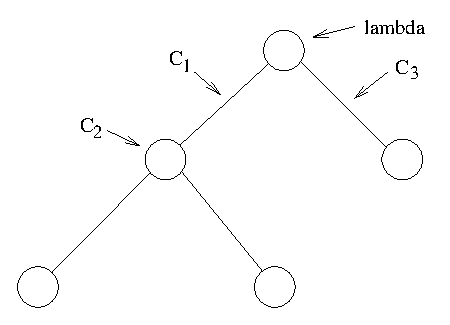
\epsfig{file=Eps/contexts.eps}
  \caption{All possible types of contexts. The context $\lambda$ is always in the context set. The
  contexts $C_1, C_2$ and $C_3$ are not necessarily in the same context set. For $C_1$, {\it direction}
  is greater than $-1$, but $C_1$ does not decode a suffix. For $C_2$, {\it direction} equals $-1$.
  Finally, for $C_3$, {\it direction} is greater than $-1$ and $C_3$ decodes a suffix.}
  \label{fig:contexts}
\end{figure}

The string $s$ can be retrieved by calling the method {\it getL} from any given context.


In the java implementation, a set of contexts, {\it contextSet}, is returned each time a new symbol
is added to the suffix tree.
\end{document}
